\chapter{测量长度}\label{ch:g2:measuring-length}

两扇门分别在两座不同的房子里：哪一扇更高？
你不能把门搬到城的另一头去和另一扇门比。
去年我们学过并排比较东西；今年我们要学科学中最伟大的一招——
把长度变成一个可以远行的\emph{数}。

\section{不用数字的比较}

\begin{example}[并排比较]\label{ex:g2:measuring-length:sidebyside}
要比较两支铅笔哪支更长，就把它们并放在桌上：伸出来更多的那支就更长。
要比较你和朋友的身高，
就背靠背站好。这个办法非常好用，
但前提是两样东西能够并放在一起。
\end{example}

\begin{example}[细绳的办法]\label{ex:g2:measuring-length:string}
两扇门碰不到一起，但一根细绳可以同时“到达”两扇门。把细绳拉直，
横跨第一扇门，剪下恰好与门等高的一段。把这段细绳
带到第二扇门旁：如果细绳不够长，
说明第二扇门更高。细绳把第一扇门的高度带过了城。
再进一步：能不能把高度装进一封
\emph{信}里寄出去？要做到这一点，我们需要数字。
\end{example}

\section{用步和拃来测量}

\begin{definition}[测量长度]\label{def:g2:measuring-length:measure}
要\emph{测量}\index{测量}一段长度，就是数一数
选定的\emph{单位}\index{单位}——一步、一拃、一根小木棍——
沿着这段长度首尾相接、既无空隙也无重叠地能排下多少个。
结果是若干个单位的数：“这个房间长 $12$ 步。”
\end{definition}

\begin{example}[试一试：量房间]\label{ex:g2:measuring-length:pace}
用脚跟贴脚尖的步子走遍你的卧室，数一数自己的脚长。请大人
也这样量一量。你可能数出 $18$ 只脚，而大人只数出 $12$ 只——
量的是\emph{同一个房间}！谁也没有数错：你的
脚比较短，所以能排下更多只。用
\emph{我}的脚量出的结果，不能用\emph{你}的脚来检验。
\end{example}

\begin{omfigure}
\begin{tikzpicture}[scale=0.8]
  \draw[thick] (0,1.6) -- (9,1.6);
  \foreach \i in {0,...,11} {
    \draw[omDef, thick] (\i*0.75,1.6) rectangle ++(0.75,0.28);
  }
  \node[right, font=\small] at (9.2,1.74) {小朋友：$12$ 只小脚};
  \draw[thick] (0,0) -- (9,0);
  \foreach \i in {0,...,7} {
    \draw[omThm, thick] (\i*1.125,0) rectangle ++(1.125,0.28);
  }
  \node[right, font=\small] at (9.2,0.14) {大人：$8$ 只大脚};
\end{tikzpicture}

{\small 同一面墙，用两种脚各量一遍：$12$ 只小脚，或 $8$ 只大脚。
脚不同，数字就不同——墙并没有变。}
\end{omfigure}

\begin{remark}[集市上的争论]\label{rem:g2:measuring-length:argument}
很长一段时间里，人们确实用脚、拇指和臂展来量东西，
集市上常常争吵不休：是谁的脚？是高个子商人的，
还是矮个子顾客的？后来各地达成的共识是
世界各地同意的办法，是为所有人选择\emph{一个}单位——
一个不属于任何人身体的单位。
\end{remark}

\section{厘米和米}

\begin{definition}[厘米和米]\label{def:g2:measuring-length:units}
\emph{厘米}\index{厘米}（写作 \unit{cm}）是一个小单位，
大约与指甲盖的宽度相当，每把尺子上都印着它。
\emph{米}\index{米}（写作 \unit{m}）是一个大单位，
恰好等于 $100$ 厘米，相当于一大步的长度。
这些单位对地球上的每个人都一样：你的
\qty{20}{cm} 和我的 \qty{20}{cm} 恰好相等。
\end{definition}

\begin{omfigure}
\begin{tikzpicture}[scale=0.85]
  \draw[thick] (0,0.5) rectangle (10,1.1);
  \foreach \i in {1,...,9} {
    \draw (\i,0.5) -- (\i,0.85);
  }
  \node[below, font=\small] at (0,0.4) {$0$};
  \node[below, font=\small] at (5,0.4) {$50$};
  \node[below, font=\small] at (10,0.4) {$100$};
  \node[above, font=\small] at (5,1.35)
    {$100$ 小段 \unit{cm} 合起来就是 \qty{1}{m}};
\end{tikzpicture}

{\small 一根米尺：一百厘米排成一行。刻线
让我们不必一个一个数，就能很快数清楚。}
\end{omfigure}

\begin{method}[用尺子测量]\label{met:g2:measuring-length:ruler}
\begin{enumerate}
  \item 把尺子沿着物体放好，紧贴物体；
  \item 把尺子的\emph{零刻度}恰好对准物体的一端，
        对准的是尺上的 $0$，而不是尺子的边缘；
  \item 读出物体另一端所对的数：
        这个数就是以厘米为单位的长度。
\end{enumerate}
若末端落在两个刻度之间，可以说“在 \qty{7}{cm} 和
\qty{8}{cm} 之间，更接近 $8$”——老老实实的话，胜过编造的数字。
\end{method}

\begin{omfigure}
\begin{tikzpicture}[scale=0.85]
  \draw[thick] (0,0) rectangle (8.4,0.7);
  \foreach \i in {0,...,12} {
    \draw (0.2+\i*0.65,0) -- (0.2+\i*0.65,0.3);
    \node[below, font=\footnotesize] at (0.2+\i*0.65,0) {\i};
  }
  \draw[thick, fill=omMeth, fill opacity=0.5]
    (0.2,1.0) rectangle (5.4,1.45);
  \node[font=\small] at (2.8,1.22) {蜡笔};
  \draw[dashed, omExo] (0.2,0.35) -- (0.2,1.0);
  \draw[dashed, omExo] (5.4,0.35) -- (5.4,1.0);
  \node[above, font=\small] at (5.4,1.5) {读数为 $8$：\qty{8}{cm}};
\end{tikzpicture}

{\small 读尺时：把零刻度对准蜡笔的一端，
读出另一端的刻度。这支蜡笔长 \qty{8}{cm}。}
\end{omfigure}

\begin{omfigure}
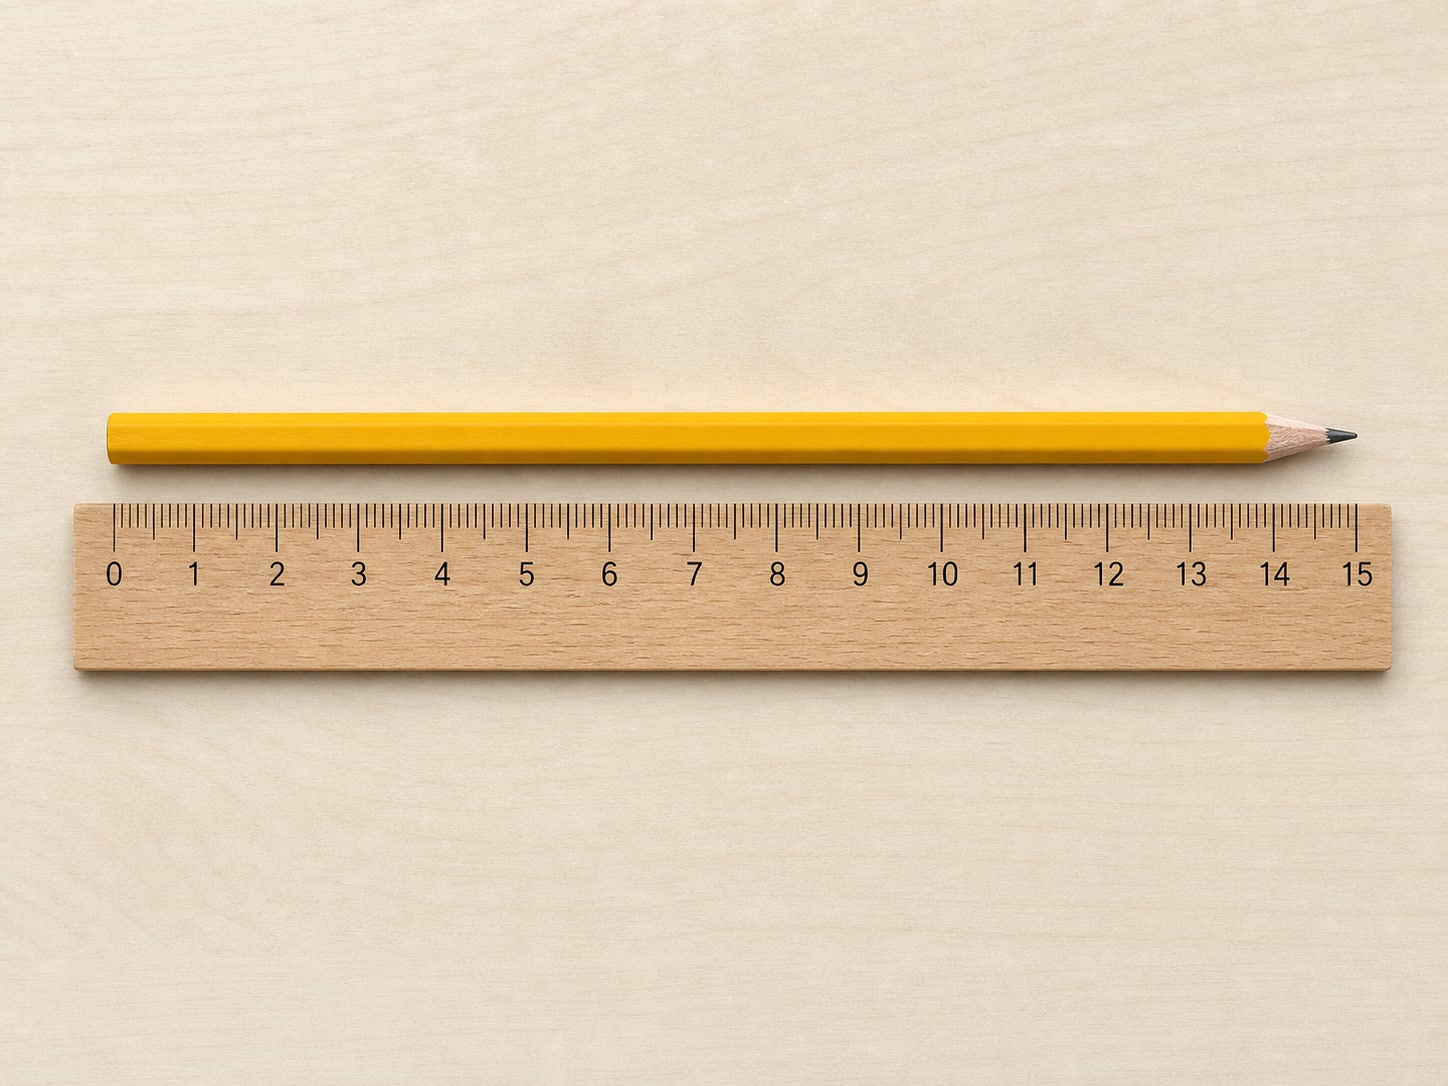
\includegraphics[width=0.52\linewidth]{images/book1/ai/g2-measuring-ruler.jpg}

{\small 正确的测量：铅笔的一端恰好对准尺子的零刻度。}
\end{omfigure}

\begin{example}[该用哪种单位？]\label{ex:g2:measuring-length:whichunit}
甲虫、邮票或你的手这样的小东西，用
厘米来量。走廊、公共汽车或游泳池这样的大东西，
用米来量：游泳池长 \qty{25}{m} ——想想看，
用指甲宽来数可太费劲了！选择合适的单位，
就占了测量工作的一半。
\end{example}

\begin{example}[先估计，再检验]\label{ex:g2:measuring-length:estimate}
测量之前，小朋友先猜一猜：厨房的餐桌有多长？
爸爸说 \qty{2}{m}，丽娜说 \qty{1}{m} 多一点。然后用米尺
来判定：\qty{1}{m} 多将近半米——丽娜猜对了。
先猜后量，既锻炼眼力，也让大家实事求是。
\end{example}

\section{练习}

\begin{exercise}[$\star$]\label{exo:g2:measuring-length:1}
不用任何尺子，你怎样比较你和朋友的身高？
那么，如果朋友住在另一个镇上，又该怎样比较？
\end{exercise}

\begin{exercise}[$\star$]\label{exo:g2:measuring-length:2}
玛拉用步数量教室，得到 $20$；她的老师
得到 $14$。谁数错了？请说明理由。
\end{exercise}

\begin{exercise}[$\star$]\label{exo:g2:measuring-length:3}
厘米与脚长或手掌跨度相比，有什么特别之处？
人们为什么要共同约定使用它？
\end{exercise}

\begin{exercise}[$\star$]\label{exo:g2:measuring-length:4}
哪个单位更合适，\unit{cm} 还是 \unit{m}：蚂蚁的长度；
\ 门的高度；\ 学校操场的长度；
这本书的宽度？
\end{exercise}

\begin{exercise}[$\star$]\label{exo:g2:measuring-length:5}
蒂姆把尺子的边缘——而不是零刻度——对准铅笔的
一端，读出 \qty{13}{cm}。他的铅笔真的长
\qty{13}{cm} 吗？他忘记了
\cref{met:g2:measuring-length:ruler}中的哪一点？
\end{exercise}

\begin{exercise}[$\star$]\label{exo:g2:measuring-length:6}
用尺子量一量：你手的宽度；\ 勺子的
长度；\ 杯子的高度。每个答案都要写上单位。
\end{exercise}

\begin{exercise}[$\star$]\label{exo:g2:measuring-length:7}
一扇门高 \qty{2}{m}。这是多少厘米？（记住：
\qty{1}{m} 等于 $100$ \unit{cm}。）
\end{exercise}

\begin{exercise}[$\star$]\label{exo:g2:measuring-length:8}
先猜一猜，再量一量：你的床有多少米长？
你猜的数字是偏大、偏小，还是差不多？
\end{exercise}

\begin{exercise}[$\star\star$]\label{exo:g2:measuring-length:9}
一条丝带长 \qty{45}{cm}，另一条长 \qty{38}{cm}。哪条
更长，相差多少厘米？能不能
在\emph{不用}数字的情况下判断？哪种方式写信更方便？
\end{exercise}

\begin{exercise}[$\star\star$]\label{exo:g2:measuring-length:10}
爷爷说：“我的花园长 $30$ 步。”请温和地向爷爷解释
为什么“$30$ 步”不能让别人核对，
并告诉他应该改用什么。如果一个小朋友
同样用步子量这个花园，会怎样？
\end{exercise}
